% !TEX root = ../paper.tex

\section{Introduction}						% 2-3 pages

%%%	Introduction: the "why" section (2-3 pages)
%%%	*	Start with a broad picture of the problem you have chosen to study and why it is interesting.
%%%	*	Provide a brief review of pertinent scientific literature, describe what information is missing and how your work addresses this gap in the literature.
%%%	*	Previous relevant publications and patents must be properly cited in the text of the Research Report and included in the Reference section of your report.
%%%	*	Describe the specific problem to be solved, the research question to be answered, the hypothesis(es) to be tested, or the product to be developed (if any).
%%%	*	Provide a brief rationale for the research, and why the work is important.







% Brief
% Try to put a lot of citations here since it is a brief
\textbf{Using our sub-\$500 unmanned aerial vehicles (UAVs), we can save thousands of victims of floods, earthquakes, hurricanes and other disasters with faster and more effective response.} We created a hardware and software platform to produce aerial maps for first responders. 3D indoor models are sent to remote doctors for victim diagnosis. Victims are automatically detected so rescuers can be quickly dispatched to people in need.

\begin{figure}[H]
	\begin{minipage}{.5\textwidth}
		\caption{Flying quadrotor UAV \cite{Wiki:ARDrone}}
		\centering
			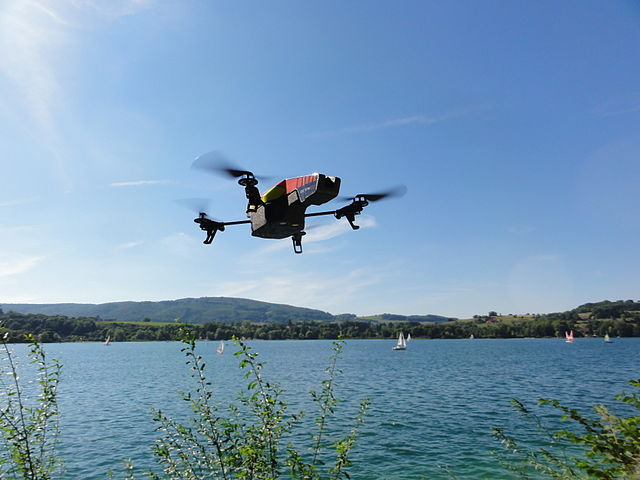
\includegraphics[width=0.95\linewidth]{illustrations/ardrone}
	\end{minipage}
	\begin{minipage}{.5\textwidth}
		\caption{Mounted phone imaging unit}
		\centering
			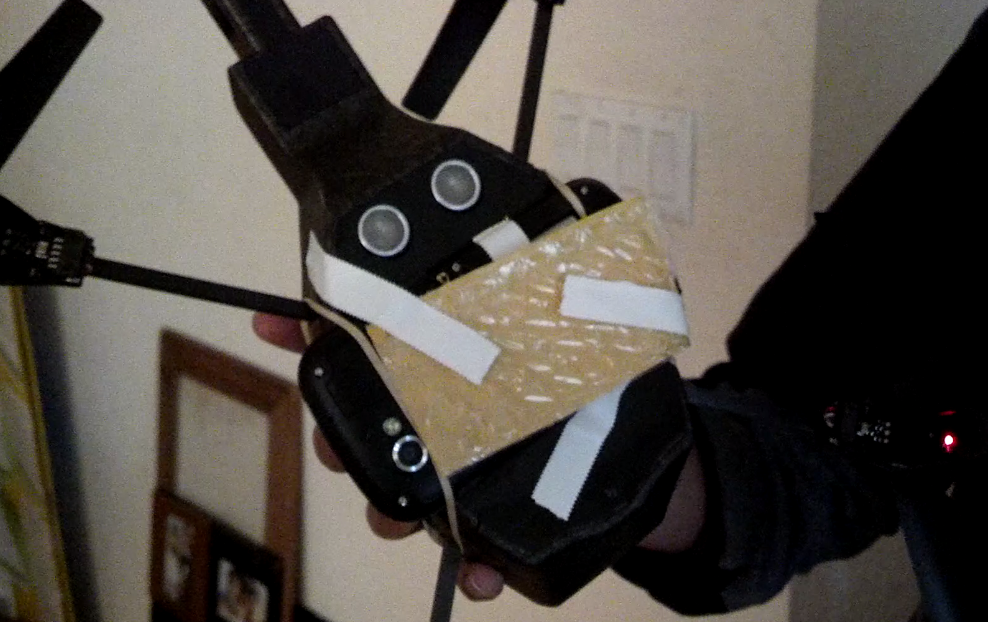
\includegraphics[width=0.95\linewidth]{illustrations/mounted}
	\end{minipage}
\end{figure}

\subsection{Brief}


\subsubsection{Project Components} % what else should this be?
\begin{description}
	\item[Autonomous Quadrotor UAV for Aerial Imaging] progressively captures up to $5 cm$ resolution aerial imagery suitable for facial recognition for under $\$500$
	\item[Agile Quadrotor for Indoor 3D Mapping] maps the interiors of buildings too dangerous to enter with a consumer level 3D camera
	\item[Central Image Processing Server] that all drones communicate with. \textit{Stitches images}, \textit{assembles 3D point clouds}, and \textit{controls the drone network}
	\item[Rapid multi-pass facial recognition] can process gigabytes of high resolution imagery to locate victims performantly
\end{description}


% Brief Aerial Mapping
\subsubsection{Problem: Aerial Mapping}
\noindent
During Hurricane Sandy and the Boston bombings, first responders used commercial level aerial imagery to coordinate search and rescue efforts. \cite{Martinez:BostonBombingAerialImagery} Aerial imagery is \textbf{critical to disaster response---responders can prioritize recovery efforts with increased situational awareness}. High resolution aerial imagery thereby maximizes rescue resources and helps to \textbf{save more lives}. By far, the most commonly used tool currently is Google Earth, however with extremely low resolutions ranging from 1m to 15m making \textit{\textbf{current imagery inadequate}}. \cite{Google:GoogleEarthSpec}

\noindent
Even with high resolution maps, responders need immediate, up-to-date maps to locate damaged areas; this requirement makes any mapping technology that is not real-time or rapidly deployable inapplicable. % chose a different word for inapplicable as satellite is still useful, it just does not solve the problem at hand
% The only applicable technology left is the use of aircraft to survey the area; however, this is expensive, requires trained operator and only offers limited awareness making it difficult to collaborate.
With current imagery and mapping technology, \textbf{automated search for survivors is infeasible}.


% Brief Indoor Searches
\subsubsection{Problem: Indoor Victim Search and Rescue}
\noindent
\textbf{First responders risk their lives} when entering buildings to search for victims. In situations where the disaster involves hazardous agents, like the Fukushima Nuclear Disaster, \textbf{searching for victims may not be possible} given the risk to responders. % cite needed

%Significant prior work has been completed on facial recognition and is very accurate with Haar cascades. % cite needed
%However, such algorithms like the Viola Jones algorithm are relatively slow and are impractical on embedded hardware such as the ARM platform, used to power the imaging UAV in this project.

\subsubsection{Potential Application: Fully Integrated Automated Victim Search in a Disaster}
\noindent
With the high resolution aerial imaging platform developed in this project, \textbf{automatic search for victims has been created, freeing disaster responders to rescue identified targets while removing the need to search indoors. Preliminary results can be available within 15 minutes, upon which a UAV autonomously deploys, images a target and returns}. 




%\subsection{Problem and Potential Applications}
%Aerial searches were used to find the Boston Marathon bomber - however, this effort required many trained police or military pilots to fly specially equipped helicopters in parallel. %CITE	

%This project created a novel system of intelligent drones that act as a group to map and analyze entire cities in real-time. Using a multi-pass approach, we generate imagery that is up to \textbf{an order of magnitude higher resolution than the best available satellite maps}. Each individual drone costs under \$500.

%We created a facial recognition algorithm designed to detect faces quickly in very large images and panoramas. Our system of drones automates victim search and can greatly improve the disaster response process.

%After mapping out a city, drones semi-autonomously generate 3D maps of the interiors of buildings, \textbf{enabling remote diagnosis of victims without endangering first responders}.


\subsection{Motivation - Potential Utility for Rapid Drone based Imagery}
Fresh aerial imagery allows first responders to target highly damaged areas quickly and prioritize rescue efforts. By shifting the time first responders spend searching for victims to rescuing them, more lives can be saved, especially with time critical injuries such as blood loss.

%We created a hardware and software platform to produce aerial maps for first responders.
%Images taken by a high-altitude drone and smartphone are analyzed to identify interest areas and low-altitude drones procure high-resolution imagery.


\subsection{Alternate Solutions}
Unmanned Aerial Vehicles (UAVs) have occasionally been used in search and rescue efforts. However, current imaging approaches have many limitations. Existing models like the Mikrokopter and Aeryon Scout (\autoref{fig:AeryonPhoto}) require direct human control, and video captured needs to be analyzed by operators. Further, these solutions are cost prohibitive (Aeryon Scout is over \$100,000). \cite{aeryonscout:price}

%\begin{wrapfigure}{R}{0.3\textwidth}
%	\caption{Aeryon Scout Pro, $\$107,500$ \cite{aeryonscout:price,Dkroetsch:AeryonPhoto}}
%	\label{fig:AeryonPhoto}
%	\vspace{-3ex}
%	\begin{center}
%		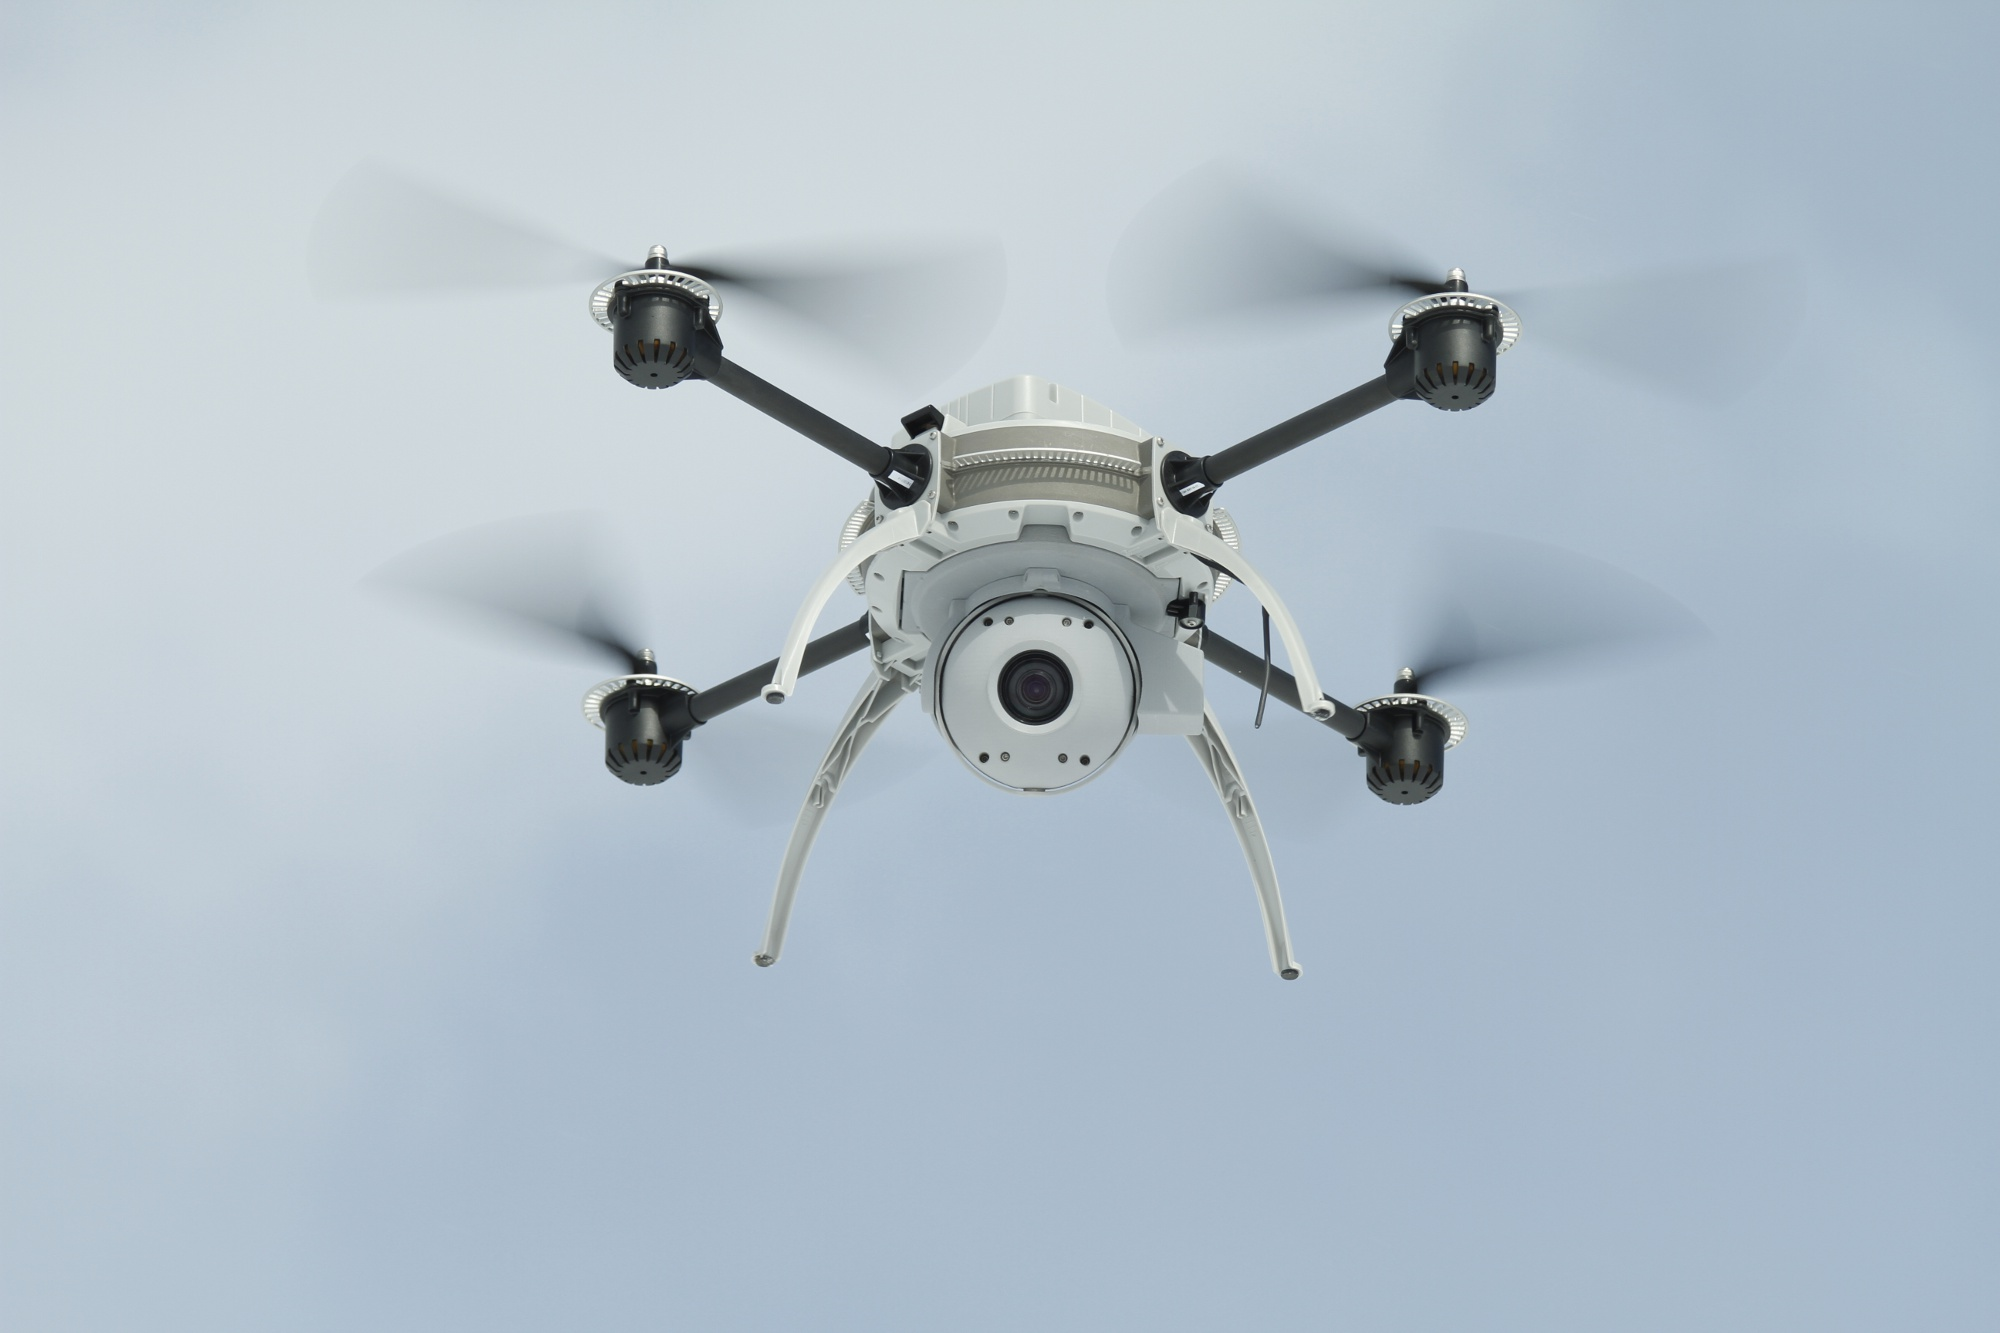
\includegraphics[width=0.29\textwidth]{illustrations/alternate_solutions/uav}
%	\end{center}
%\end{wrapfigure}

Satellites such as GeoEye-I can take 8-10 days to reach the disaster area, post-storm cloud fields can obstruct clear view, and non-military satellite imagery has a capped resolution at $\frac{1}{2}$ meter at best, often at a resolution as low as $15m^2$ per pixel. \cite{Shankland:GeoEyeImagery}

Commercial drones typically range from $\$10,000$ to over $\$100,000$ while providing little additional value for rescue teams as most lack autonomous capabilities, requiring a specially trained operator, making such drones cost-prohibitive for many organizations.
\cite{Campoy:CommercialDronesExpensive}

\subsection{Quadrotor Advantages}
\vspace{1ex}
\begin{onehalfspacing}
	\begin{itemize}
		\item Quadrotors are similar to helicopters but have more maneuverability meaning quadrotors can hover in place, extremely important for aerial photography.
		\item Diametrically opposite blades rotate in the same direction, with one set rotating clockwise and one rotating counter-clockwise.
		\item The counter rotation of adjacent blades results in no net torque on the quadrotor.
		\item VTOLs (Vertical Takeoff and Landing): Drones can launch and land in confined spaces on many terrains
		\item Reduced mechanical complexity means safer and lower cost than helicopters
	\end{itemize}
\end{onehalfspacing}

\subsection{Project Goals}
Our engineering goal is the design and construction of an \textit{affordable} autonomous quadrotor based aerial photography system for rapid acquisition of accurate and up-to-date maps to aid disaster response or commercial interests coupled with indoor 3D scanning to allow responders to locate victims in a damaged building.

\subsection{Engineering Design Criteria}
\vspace{1ex}
\begin{onehalfspacing}
	\begin{enumerate}
		\item Function with daytime environments, winds under 20 km/h
		\item Include GPS and other sensors for navigation
		\item Individual unit less than \$500
		\item High resolution front and bottom cameras to ensure quality imagery.
		\item The UAV should have an angular resolution better than 41cm to beat current satellite imaging technology
	\end{enumerate}
\end{onehalfspacing}

\subsection{Team Contributions}
Team Leader primarily focused on the construction of the quadrotor platform as well as the design and architecture of the distributed server cluster. This included the control systems that drove the quadrotor. Team Leader designed the 3D indoor iteration of the quadrotor which utilized a very heavily modified consumer RGB-D 3D sensor.
Team Member created the image processing toolset and built the 3D stitching pipeline to generate point clouds for interiors of buildings.
